\section{Server}
\begin{figure}[h]
	\centering
	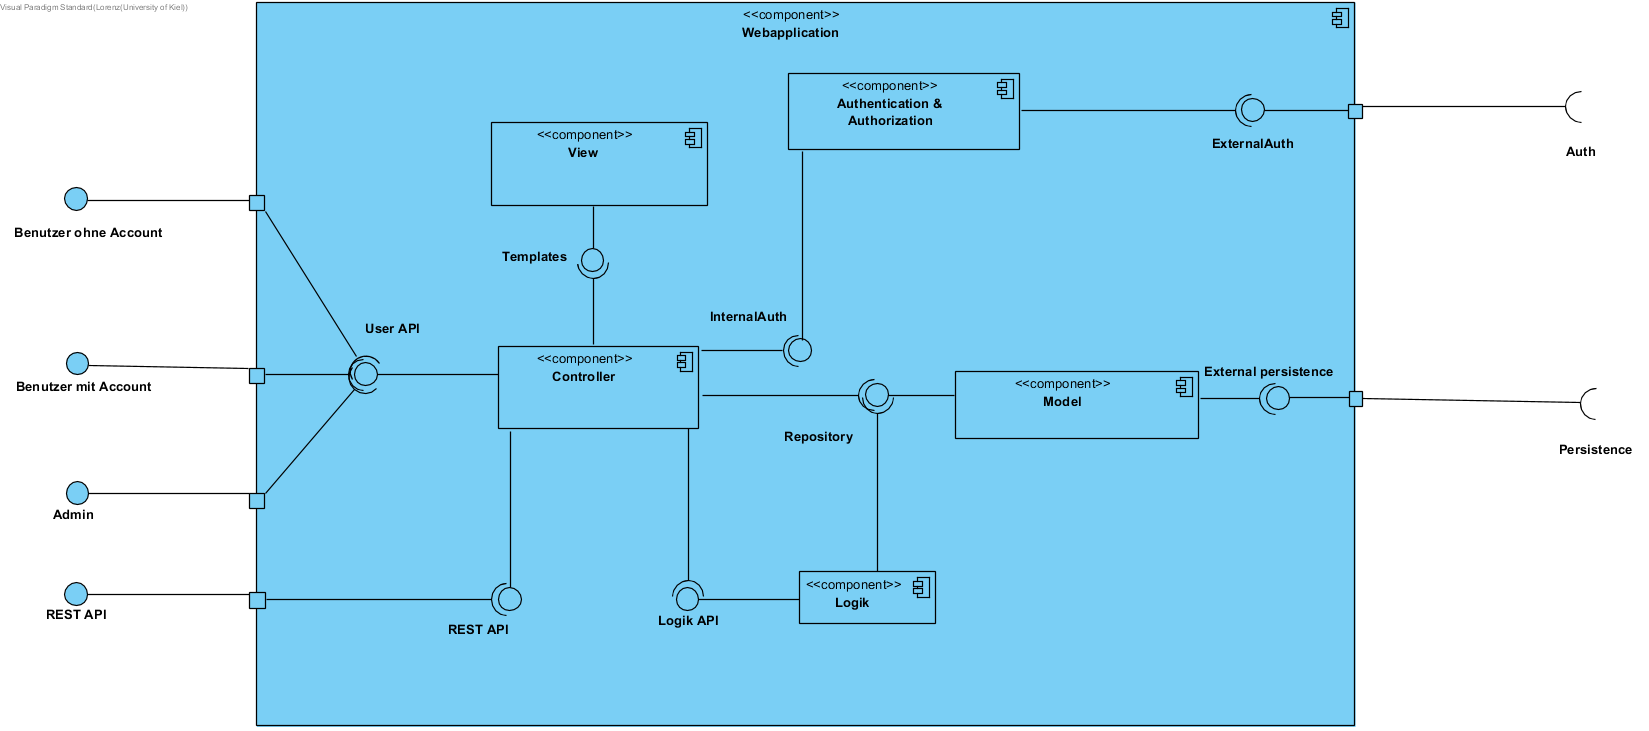
\includegraphics[width=\textwidth]{komponentendiagramm/Server}
	\caption{Komponentendiagramm - Server}
	\label{fig:komponentendiagramm-server}
\end{figure}

\begin{table}[h]
	\centering
	\begin{tabularx}{\textwidth}{X X}
		\rowcolor[HTML]{C0C0C0}
		\textbf{Komponentenname} & \textbf{Aufgabe} \\
		Authentification \& Authorization & Authentifizierung und Logins/Logouts\\
		\rowcolor[HTML]{E7E7E7}
		Controller & Beantwortet Anfragen von außen und übernimmt die interne Kommunikation\\
		Logik & Berechnet Lösungen für Anfragen, die über die einfache Logik des Controllers hinaus geht\\
		\rowcolor[HTML]{E7E7E7}
		Model & Enthält alle Daten aus der DB und bietet sie über eine Schnittstelle an\\
		View & View bereitet die Daten in einer HTML Seite auf und enthält Funktionalität für die Webseite
	\end{tabularx}
	\caption{Subkomponentenbeschreibung - Server}
	\label{table:Subkomponentenbeschreibung - server}
\end{table}

\FloatBarrier
Die meisten Schnittstellen aus dieser Abbildung werden bereits durch das Spring-Framework bereitgestellt.
In diesem System stellen die Webseitennutzer über die User API Anfragen an den Controller.
Die App-Nutzer nutzen dafür die REST API.
Der Controller wertet die Anfrage aus und bearbeitet diese mit Hilfe der anderen Komponenten.
Dabei ist die Authentification \& Authorization-Komponente dafür zuständig, zu überprüfen ob eine Anfrage authentifiziert ist und auch für Logins und Logouts.
Die View-Komponente ist hier bei für die Aufbereitung der Informationen in HTML zuständig. Weiter ist dort Funktionalität/Logik für die Browserwebseite mit enthalten.
In der Logik-Komponente werden komplexere Berechnungen durchgeführt.
So werden hier beispielsweise Alternativen für inkompatible Verbindungen.
Die Model-Komponente ist lediglich für die Datenverwaltung und die Kommunikation mit der DB zuständig.
Dafür stellt die Model-Komponente die Repository-Schnittstelle bereit.

\section{App}
\begin{figure}[h]
	\centering
	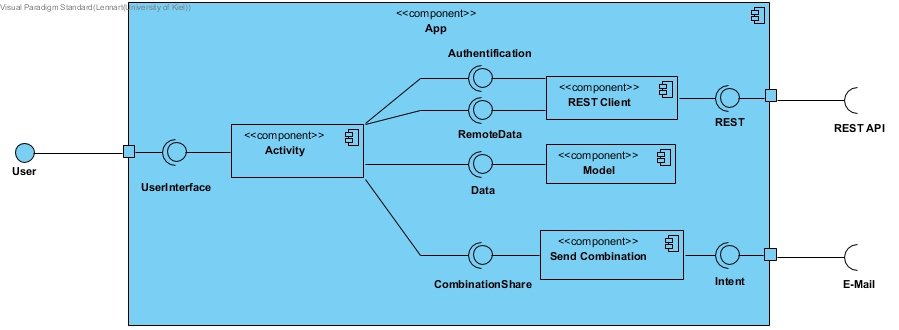
\includegraphics[width=\textwidth]{komponentendiagramm/App}
	\caption{Komponentendiagramm - App}
	\label{fig:komponentendiagramm-app}
\end{figure}

\begin{table}[h]
	\centering
	\begin{tabularx}{\textwidth}{X X}
		\rowcolor[HTML]{C0C0C0}
		\textbf{Komponentenname} & \textbf{Aufgabe} \\
		Activity & Darstellung der App Oberflächen und Schnittstelle für den Benutzer\\
    \rowcolor[HTML]{E7E7E7}
		 Model & Modelliert die Daten, die von der REST API zur Verfügung gestellt werden\\
		 REST Client & Kommunikation zwischen REST API und der App\\
    \rowcolor[HTML]{E7E7E7}
		Send Combination & Generiert PDF und leitet dies weiter an Standard E-Mail Programm
	\end{tabularx}
	\caption{Subkomponentenbeschreibung - App}
	\label{table:Subkomponentenbeschreibung - app}
\end{table}

Die App Komponente modelliert die zu entwickelnde App.
Der User interagiert dabei über das User Interface mit der Anwendung.
Die Activity Komponente nimmt dabei die Interaktionen entgegen und führt dementsprechend Aktionen aus.
Dabei besteht die Activity Komponente aus der Darstellung, die bei Android über XML stattfindet und den eigentlichen Activities, die die Interaktionen entgegennehmen.
Von den Activities aus werden die REST Client, Model und Send Combination Komponenten verwendet.
\\
Der REST Client bietet einerseits eine Schnittstelle für die Authentifikation und für das Einloggen und anderseits eine, um Daten von dem Server zu holen.
\\
Die Model Komponente modelliert die benötigten Daten in der App.
Die Klassen im Model entsprechen den Daten von der REST API.
\\
Die Send Combination Komponente ermöglicht das Teilen von Kombinationen.
Dabei wird die Kombinationen und ein beschreibender Text zu einem PDF umgewandelt und dann über eine Schnittstelle an einen E-Mail Client weitergegeben.
